\documentclass{article}

\title{
    {\Large \textsc{MS12 -- Analyse numérique pour la diffraction à haute fréquence}} \\[15pt]
    \textbf{Implémentation de l’approximation de l’optique géométrique}
}
\author{Clément Baillet \and Armand Wayoff}
\date{\today}

\usepackage[headheight=15pt, top=20mm, bottom=20mm, left=15mm, right=15mm]{geometry}
\usepackage{fancyhdr}
\usepackage[T1]{fontenc}
\usepackage[french]{babel}
\usepackage{graphicx} 
\usepackage{subcaption}
\usepackage{float} 
\usepackage{amsmath,amssymb,amsthm,mathtools}
\usepackage{comment}
\usepackage{pgfplots}
\usepackage{pgfplotstable}
\pgfplotsset{compat=1.18}
\usepackage{booktabs}
\usepackage{hyperref}

\begin{document}

\pagestyle{fancy}
\fancyhead{}\fancyfoot{}
\fancyhead[C]{\textbf{Clément Baillet \& Armand Wayoff -- TP MS12}}
\fancyfoot[C]{\textbf{\thepage}}

\maketitle

\begin{abstract}
Dans ce projet, on implémente l'approximation de l’optique géométrique pour un problème de diffraction haute fréquence par un obstacle convexe en dimension 2. Les quantités géométriques sont calculées sous Python, puis importées dans FreeFem++ afin de construire une approximation asymptotique du champ diffracté. Cette approximation est comparée à une solution de référence calculée par éléments finis avec une couche PML. On présente enfin une étude de l’erreur en fonction de la fréquence.
\end{abstract}

\tableofcontents

\section{Objectifs numériques}

On s’intéresse au problème extérieur de Helmholtz pour une onde plane incidente
\[
u^{\mathrm{inc}}(x)=e^{ikx_1},
\]
diffractée par un obstacle convexe \(\Omega \subset \mathbb{R}^2\).

\noindent Les objectifs numériques sont :

\begin{enumerate}
    \item visualiser la solution $S$ de l’équation eikonale;
    \item tracer des caractéristiques associées à cette équation (les rayons);
    \item tracer la partie réelle de la solution des équations de l’optique géométrique;
    \item tracer la partie réelle d’une solution de référence calculée par éléments finis (pour comparer visuellement), avec la méthode de troncature par PML;    
    \item tracer la valeur absolue de la différence entre ces deux fonctions;    
    \item calculer l’erreur en norme $L^2$ sur le domaine de calcul ``physique'' (donc en retirant la couche PML).
\end{enumerate}

\subsection{Visualisation de la solution $S$ de l'équation eikonale et tracé des caractéristiques associées à l'équation eikonale}

\begin{figure}[H]
\centering
\begin{subfigure}[t]{.5\textwidth}
    \centering
    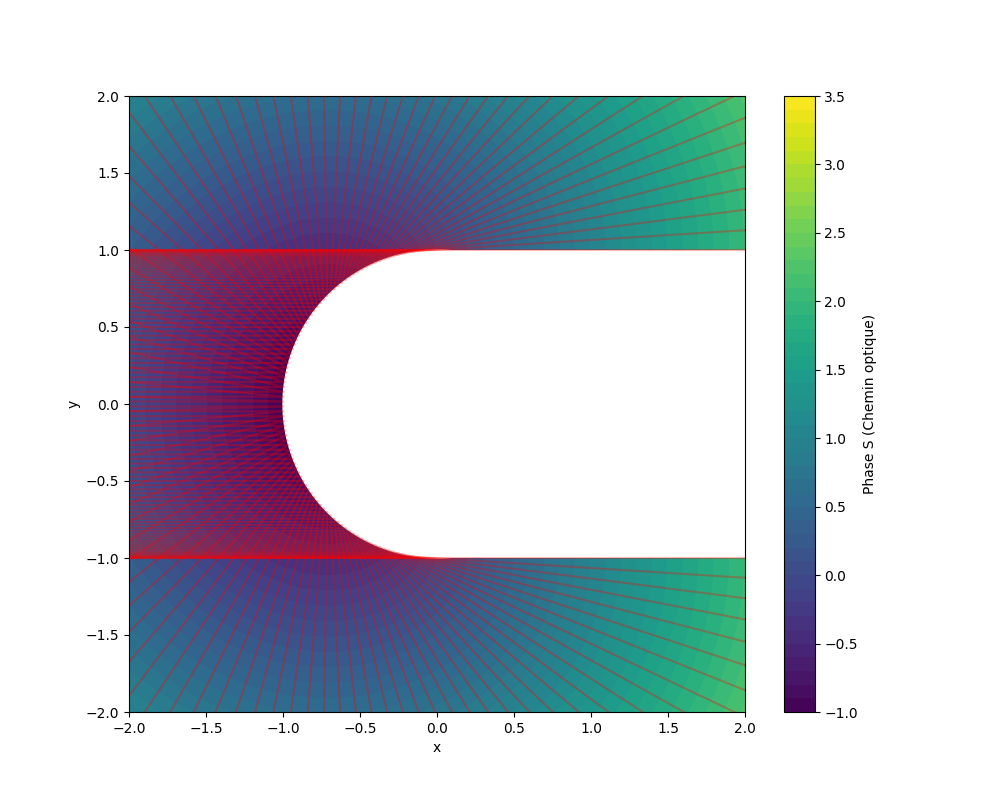
\includegraphics[width=\textwidth]{img/OG_rayons_phaseS.png}
    \caption{Disque}
\end{subfigure}%
\begin{subfigure}[t]{.5\textwidth}
    \centering
    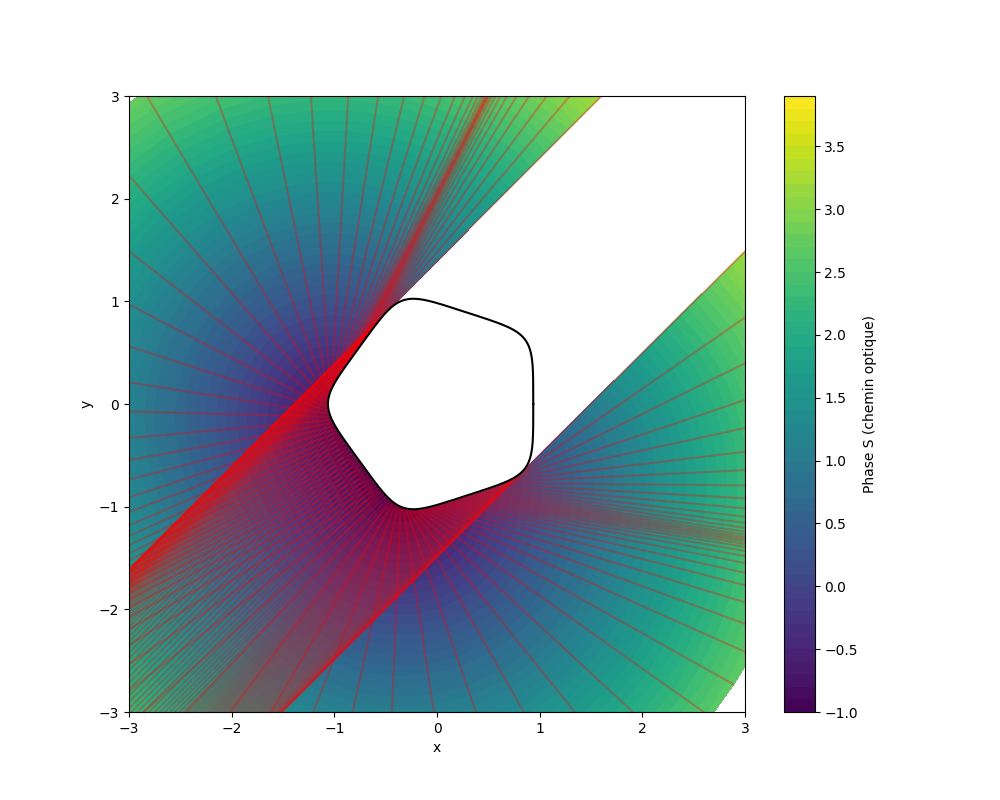
\includegraphics[width=\textwidth]{img/OG_rayons_phaseS_roundedpolygon.png}
    \caption{Polygone arrondi avec un angle d'incidence de $5\pi/4$}
\end{subfigure}
\caption{Visualisation de la solution $S$ de l'équation eikonale et tracé des caractéristiques associées à l'équation eikonale pour différentes formes d'obstacles convexes. Nombre de rayons: $100$}
\end{figure}


\begin{figure}[H]
\centering
\begin{subfigure}[t]{.5\textwidth}
    \centering
    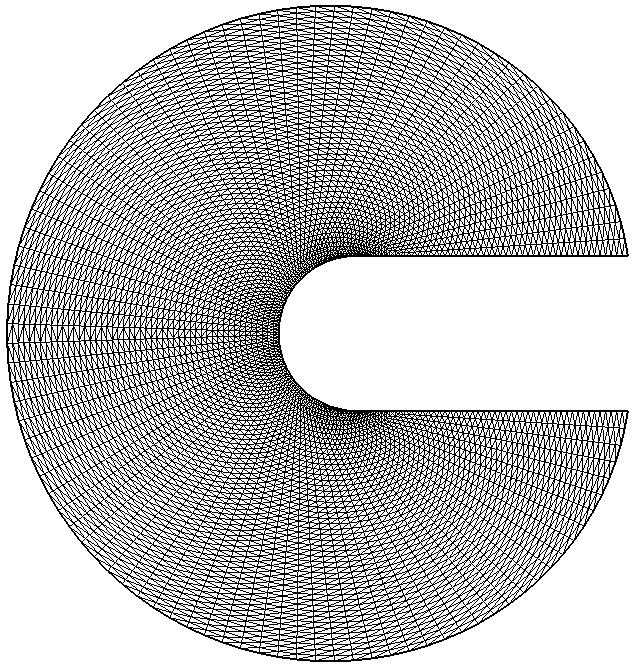
\includegraphics[width=.6\textwidth]{img/maillage_OG_python.png}
    \caption{Maillage Python pour l'approximation de l'optique géométrique. Nombre de rayons: $100$, nombre de points de discrétisation par rayon: $50$}
\end{subfigure}%
\begin{subfigure}[t]{.5\textwidth}
    \centering
    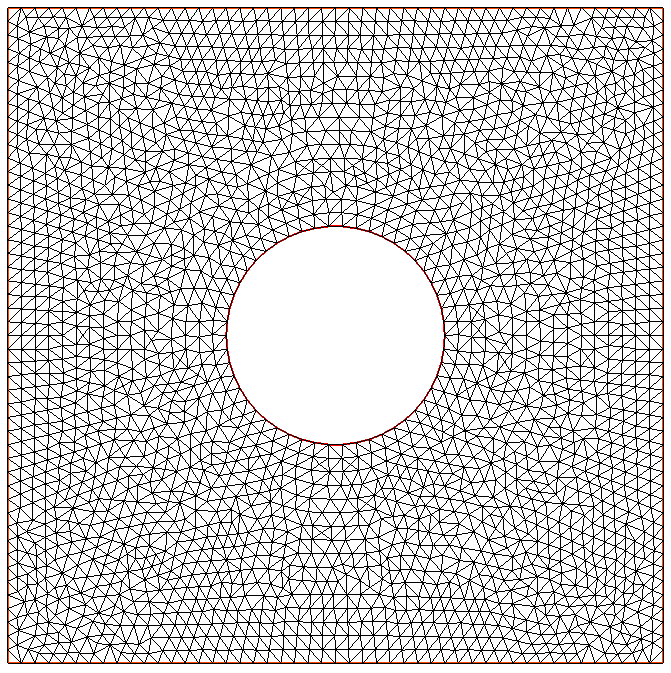
\includegraphics[width=.6\textwidth]{img/maillage_freefem.png}
    \caption{Maillage FreeFem++ pour la solution de référence. $\boxed{h = \frac{\pi}{2k}}$ avec $k = 4\pi$.}
\end{subfigure}
\caption{Visualisation des maillages utilisés pour l'approximation d'optique géométrique et la solution de référence calculée par éléments finis avec PML}
\end{figure}

\subsection{Tracé de la partie réelle de la solution des équations de l'optique géométrique}

\begin{figure}[H]
    \centering
    \begin{subfigure}[t]{.5\textwidth}
        \centering
        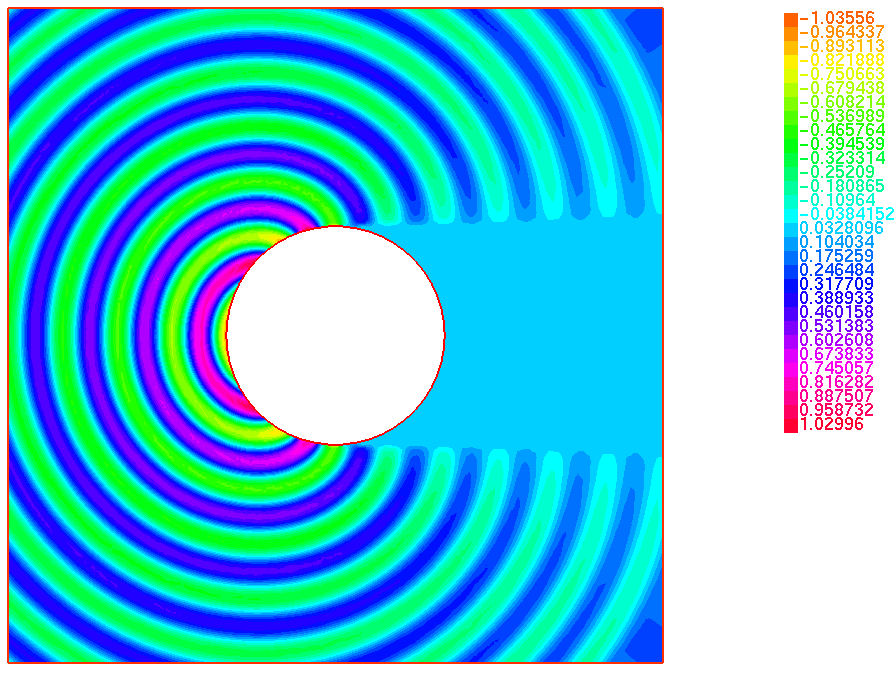
\includegraphics[width=.8\textwidth]{img/partie_reelle_champ_diff_OG.png}
        \caption{$k = 4\pi$}
    \end{subfigure}%
    \begin{subfigure}[t]{.5\textwidth}
        \centering
        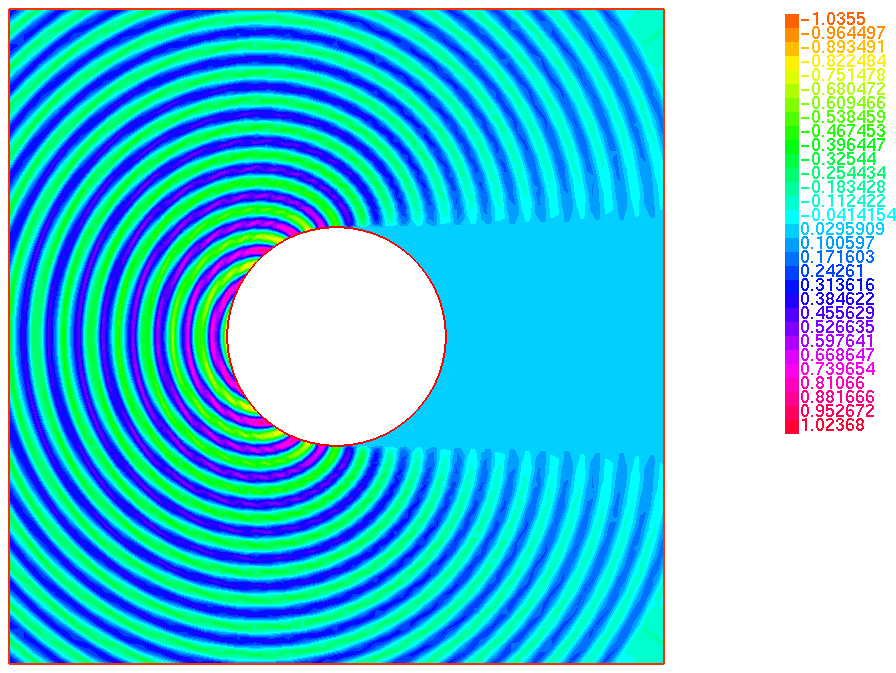
\includegraphics[width=.8\textwidth]{img/partie_reelle_champ_diff_OG_8pi.png}
        \caption{$k = 8\pi$}
    \end{subfigure} \\
    \begin{subfigure}[t]{\textwidth}
        \centering
        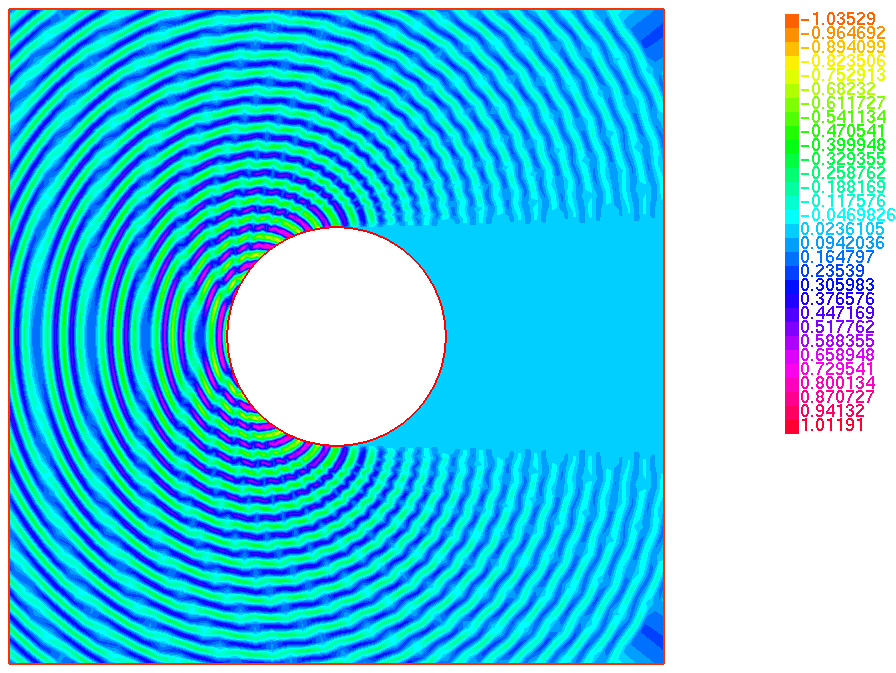
\includegraphics[width=.4\textwidth]{img/partie_reelle_champ_diff_OG_12pi.png}
        \caption{$k = 12\pi$}
    \end{subfigure}
    \caption{Partie réelle du champ diffracté par l'optique géométrique pour différentes fréquences $k$}
\end{figure}

\subsection{Tracé de la partie réelle d'une solution de référence calculée par éléments finis avec la méthode de troncature par PML}

\begin{figure}[H]
    \centering
    \begin{subfigure}[t]{.5\textwidth}
        \centering
        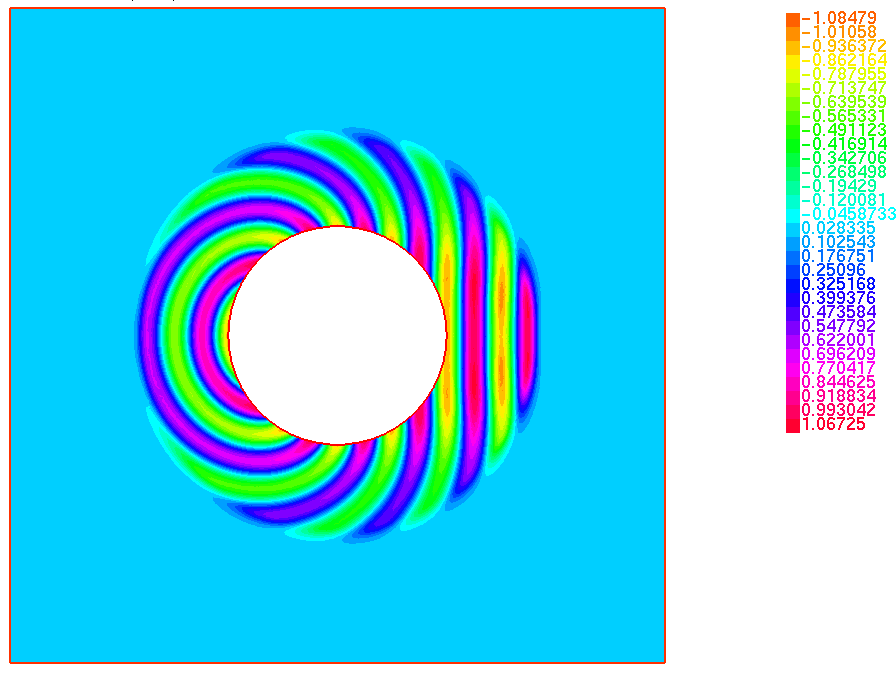
\includegraphics[width=.8\textwidth]{img/partie_reelle_champ_diff_pml.png}
        \caption{$k = 4\pi$}
    \end{subfigure}%
    \begin{subfigure}[t]{.5\textwidth}
        \centering
        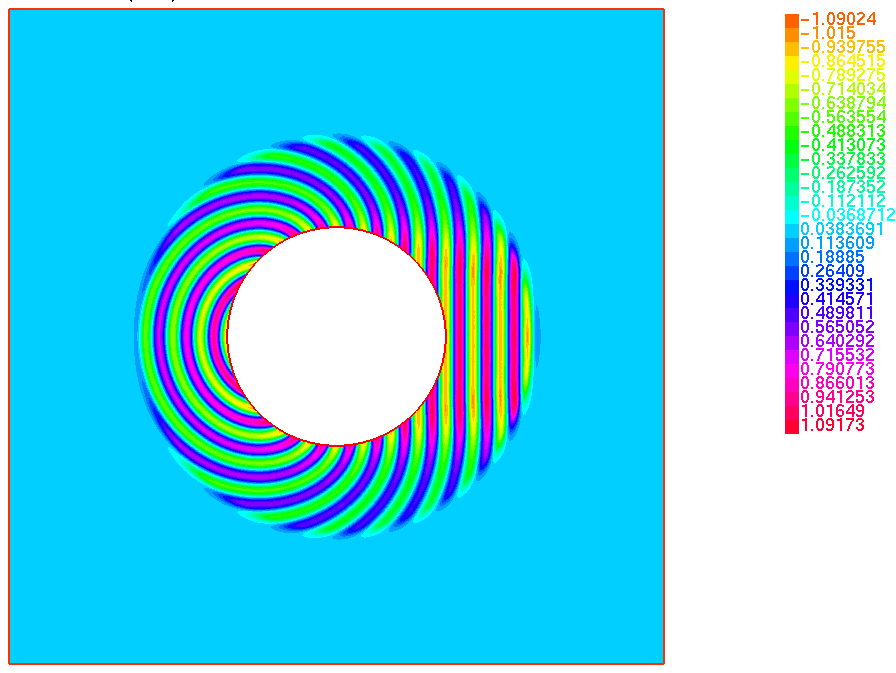
\includegraphics[width=.8\textwidth]{img/partie_reelle_champ_diff_pml_8pi.png}
        \caption{$k = 8\pi$}
    \end{subfigure} \\
    \begin{subfigure}[t]{\textwidth}
        \centering
        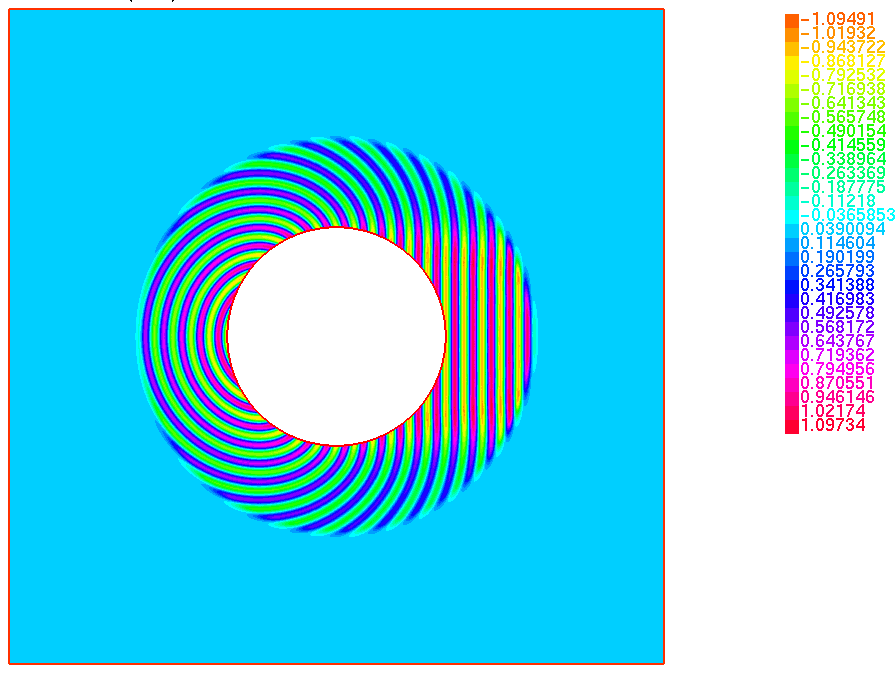
\includegraphics[width=.4\textwidth]{img/partie_reelle_champ_diff_pml_12pi.png}
        \caption{$k = 12\pi$}
    \end{subfigure}
    \caption{Partie réelle d'une solution de référence calculée par éléments finis avec la méthode de troncature par PML pour différentes fréquences $k$}
\end{figure}

\subsection{Tracé de la valeur absolue de la différence entre ces deux fonctions}

\begin{figure}[H]
    \centering
    \begin{subfigure}[t]{.5\textwidth}
        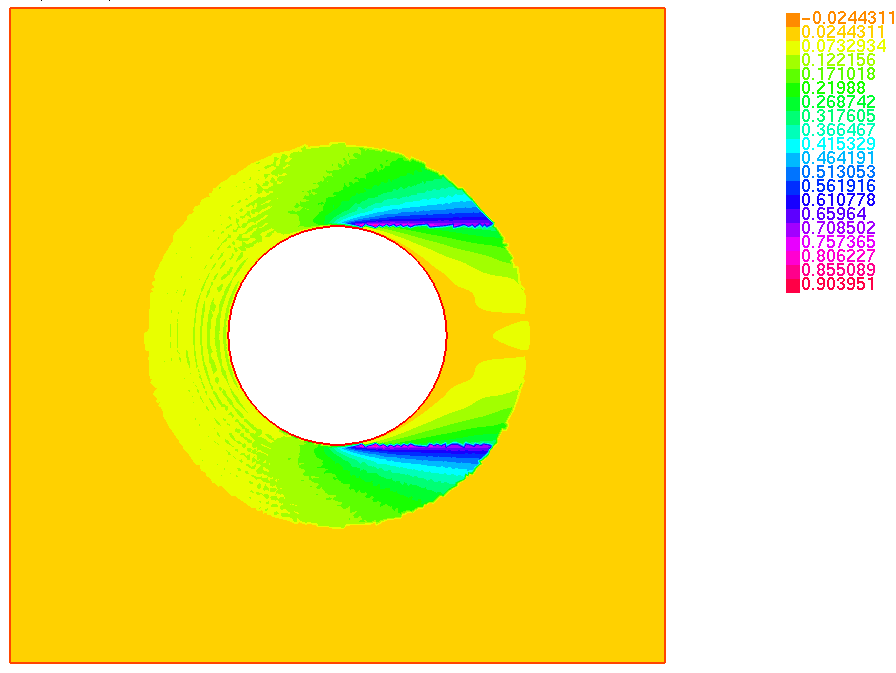
\includegraphics[width=.8\textwidth]{img/erreur_absolue_OG_PML.png}
        \caption{$k = 4\pi$}
    \end{subfigure}%
    \begin{subfigure}[t]{.5\textwidth}
        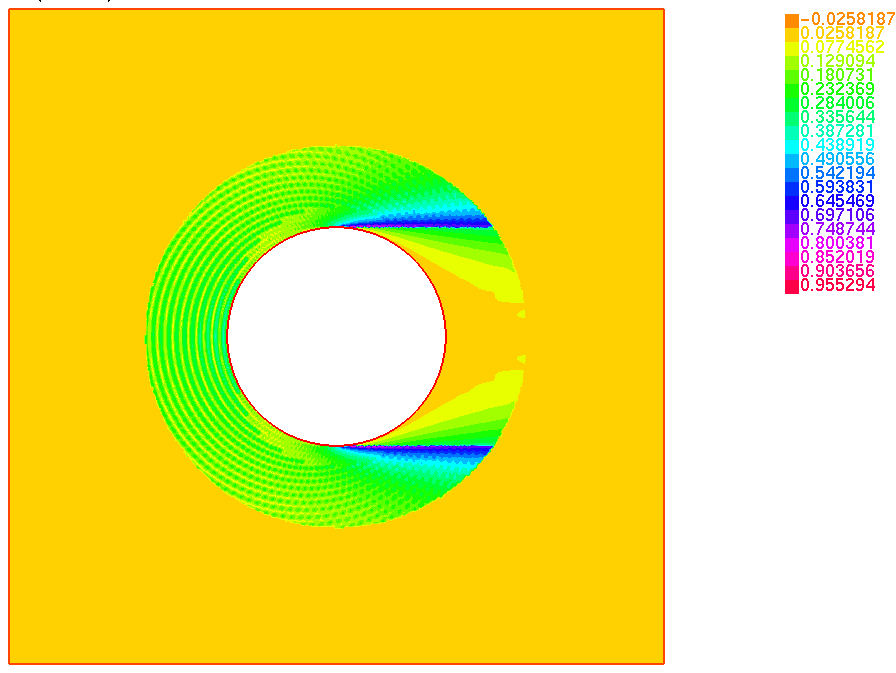
\includegraphics[width=.8\textwidth]{img/erreur_absolue_OG_PML_8pi.png}
        \caption{$k = 8\pi$}
    \end{subfigure} \\
    \begin{subfigure}[t]{\textwidth}
        \centering
        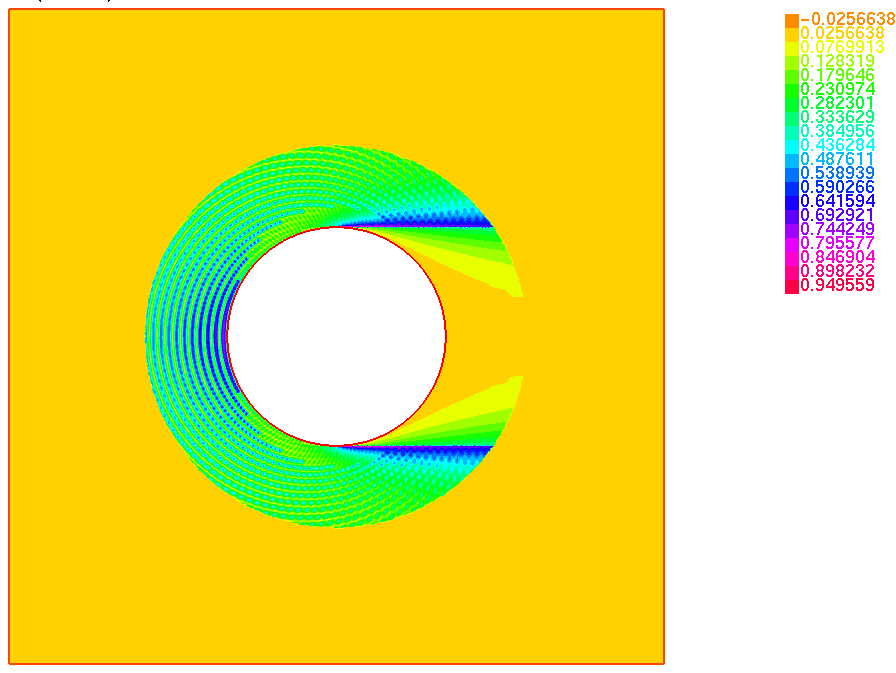
\includegraphics[width=.4\textwidth]{img/erreur_absolue_OG_PML_12pi.png}
        \caption{$k = 12\pi$}
    \end{subfigure}
    \caption{Valeur absolue de la différence entre les solutions de l'optique géométrique et de référence calculée par éléments finis avec PML}
    \label{fig:erreur}
\end{figure}

\subsection{Calcul de l'erreur en norme $L^2$ sur le domaine de calcul "physique"}

\begin{figure}[H]
    \centering
    \begin{tikzpicture}
\begin{loglogaxis}[
    xlabel={$k$},
    ylabel={},
    xtick={12.5664, 18.8496, 25.1327, 31.4159, 37.6991},
    xticklabels={$4\pi$, $6\pi$, $8\pi$, $10\pi$, $12\pi$},
    grid=major,
    height=6cm,
    width=8cm,
    legend entries={Erreur en norme $L^2$, Erreur relative en norme $L^2$},
    legend style={
        at={(0.03,1.03)},
        anchor=south west
    },
]
    \pgfplotstableread{data/erreur.dat}
        \datatable
    
    \addplot table[y = errL2] from \datatable;
    \addplot table[y = errrelL2] from \datatable;

\end{loglogaxis}
\end{tikzpicture} 
    \caption{Erreur en norme $L^2$ entre l'approximation d'optique géométrique et la solution de référence calculée par éléments finis avec PML en fonction de la fréquence $k$.}
\end{figure}

L’erreur $L^2$ et l’erreur relative augmentent avec le nombre d’onde $k$. Ce comportement est cohérent avec la théorie du problème de Helmholtz à haute fréquence. 

{\color{red}
À commenter :
\begin{itemize}
    \item les zones où l’approximation est bonne ;
    \item les zones où elle est mauvaise ;
    \item l’effet de la zone d’ombre ;
    \item la dépendance en fréquence.
\end{itemize}

\begin{itemize}
    \item \textbf{Méthode :} implémentation de l’approximation d’optique géométrique (ansatz WKB), basée sur la résolution de l’équation eikonale pour la phase et des équations de transport pour l’amplitude.

    \item \textbf{Résultats :} bonne approximation dans les zones éclairées, mais augmentation de l’erreur avec la fréquence $k$, liée à l’effet de pollution et à l’amplification par la résolvante.

    \item \textbf{Limites :} échec en zone d’ombre, discontinuités aux caustiques, absence de prise en compte des phénomènes de diffraction.

    \item \textbf{Améliorations :} utilisation de l’optique physique, corrections en zone d’ombre, et prise en compte des rayons rampants pour mieux modéliser la diffraction.
\end{itemize}

\begin{table}[H]
\centering
\begin{tabular}{ll}
\toprule
Paramètre & Valeur \\
\midrule
Obstacle & cercle de rayon 1 \\
\(x_{\min}\) & \(-2\) \\
\(\theta_{\min}\) & \(\pi/2\) \\
\(\theta_{\max}\) & \(3\pi/2\) \\
\(L\) & \(3.5\) \\
Nombre de rayons & \(100\) \\
Nombre de points par rayon & \(50\) \\
\bottomrule
\end{tabular}
\caption{Exemple de paramètres utilisés dans les calculs géométriques.}
\end{table}
}

\section{Questions théoriques}

{\color{red}
\begin{enumerate}
    \item Une fonction ayant un saut non nul n'est pas dans $H^1_\mathrm{loc}$.
    \item Comme nous l'observons sur la figure \ref{fig:erreur}, l'erreur est la plus forte près de la frontière lumière/ombre. C’est dans cette zone que l’ansatz de l'optique géométrique devient faux car il coupe artificiellement le champ, néglige les phénomènes de diffraction et ne prend pas en compte les rayons rampants. De plus, la solution est très oscillante dans cette zone, ce qui rend la résolution numérique plus difficile.
\end{enumerate}
}

\end{document}